%\documentclass{article}
%\usepackage{graphicx,subfigure}
%\begin{document}

\begin{figure}[!h]
  \centering
   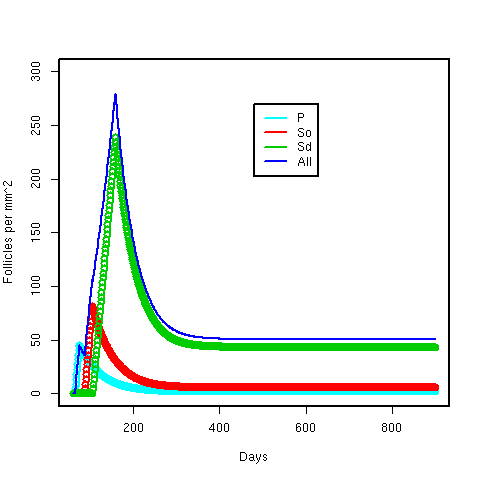
\includegraphics[width=0.9\textwidth]{basedens.png}
%  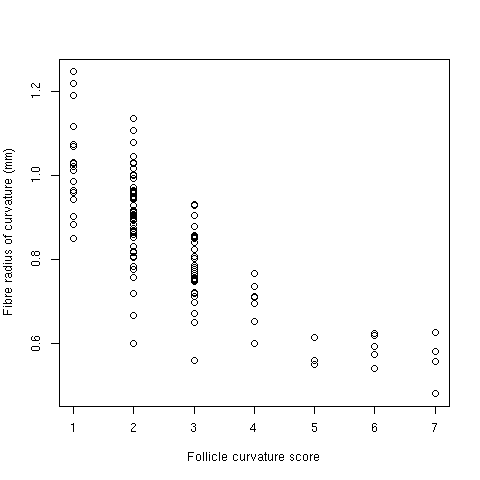
\includegraphics{ofdamm.png}
  \caption{Calculated values of follicle density at times from day 60 to day 900 from equations ~\ref{eqn:prim} to ~\ref{eqn:sd3} with values for parameters specified as for the 20 parameters of Table~\ref{tab:base}}
  \label{fig:basedens}
\end{figure}

%\end{document}

